\chapter{Appendix}

\section{Modelling time series}
\label{sec:full_reduced}
An alternative method (as to \ref{sec:mds}) to determine 
the dynamic response of a certain
gene in the network is based on the work of \cite{Mar2009}. 
Since statistical analyses of microarray time series data usually 
suffers from the lack
of replicates at each time point, classical statistical tests 
cannot be directly applied. In order to 
circumvent this problem and increase the statistical power,
previous studies~\citep{Bar-Joseph2003,Storey2005} have taken into 
account all data points at the
same time by fitting the time series with a spline function and 
performing likelihood ratio test to judge the significance of 
differential expression.

Our approach works in an analogous way.
More specifically, we fitted cubic regression models to each 
individual gene expression profile. A cubic model was chosen 
because of the moderately large number of time points 
available to fit a model with four to eight parameters. 
For a single gene, both a full model and a reduced model are 
fitted to its time-course expression profiles under the 
stimulation and control condition. The full model specifies 
a set of parameters that capture the time-dependent curvature
of a gene's expression profile for each separate condition. 
In this way, the full model assumes that the expression 
profile is different across the two conditions, or
\begin{eqnarray}
\begin{pmatrix}
Y_{control,1}\\
\cdots\\
Y_{control,N}\\
Y_{stimulation,1}\\
\cdots\\
Y_{stimulation,N}
\end{pmatrix}
%
&= \alpha_0 
\begin{pmatrix}
1\\
\cdots\\
1\\
0\\
\cdots\\
0
\end{pmatrix}
%
+ \alpha_1 
\begin{pmatrix}
t_1\\
\cdots\\
t_N\\
0\\
\cdots\\
0
\end{pmatrix}
%
+ \alpha_2 
\begin{pmatrix}
t_1^2\\
\cdots\\
t_N^2\\
0\\
\cdots\\
0
\end{pmatrix}
%
+ \alpha_3
\begin{pmatrix}
t_1^3\\
\cdots\\
t_N^3\\
0\\
\cdots\\
0
\end{pmatrix}\notag \\
%
&+ \beta_0 
\begin{pmatrix}
0\\
\cdots\\
0\\
1\\
\cdots\\
1
\end{pmatrix}
%
+ \beta_1
\begin{pmatrix}
0\\
\cdots\\
0\\
t_1\\
\cdots\\
t_N
\end{pmatrix}
%
+ \beta_2
\begin{pmatrix}
0\\
\cdots\\
0\\
t_1^2\\
\cdots\\
t_N^2
\end{pmatrix}
%
+ \beta_3
\begin{pmatrix}
0\\
\cdots\\
0\\
t_1^3\\
\cdots\\
t_N^3
\end{pmatrix}
%
+ 
\begin{pmatrix}
\epsilon_1\\
\epsilon_2\\
\cdots\\
\cdots\\
\epsilon_{2N-1}\\
\epsilon_{2N}
\end{pmatrix}
\end{eqnarray}
where $t=(t_1,t_2,\dotsc,t_N)$ corresponds to the measured time points, and
$\epsilon = (\epsilon_1,\epsilon_2,\dotsc,\epsilon_{2N})$ represents a random
normal residual error term. The parameters $\alpha_0,\alpha_1,\alpha_2,
\alpha_3$ and $\beta_0,\beta_1,\beta_2,\beta_3$ are the coefficients of the 
time covariate in the model for the control and stimulation time series 
respectively.

The reduced model, in contrast, is a simpler model that assumes the expression
profiles for different conditions need only be specified by one set of 
parameters, or 
\begin{align}
\begin{pmatrix}
Y_{control,1}\\
\cdots\\
Y_{control,N}\\
Y_{stimulation,1}\\
\cdots\\
Y_{stimulation,N}
\end{pmatrix}
%
&= \lambda_0 
\begin{pmatrix}
1\\
\cdots\\
1\\
1\\
\cdots\\
1
\end{pmatrix}
%
+ \lambda_1 
\begin{pmatrix}
t_1\\
\cdots\\
t_N\\
t_1\\
\cdots\\
t_N
\end{pmatrix}
%
+ \lambda_2 
\begin{pmatrix}
t_1^2\\
\cdots\\
t_N^2\\
t_1^2\\
\cdots\\
t_N^2
\end{pmatrix}
%
+ \lambda_3
\begin{pmatrix}
t_1^3\\
\cdots\\
t_N^3\\
t_1^3\\
\cdots\\
t_N^3
\end{pmatrix}\notag \\
%
&+ 
\begin{pmatrix}
\epsilon_1\\
\epsilon_2\\
\cdots\\
\cdots\\
\epsilon_{2N-1}\\
\epsilon_{2N}
\end{pmatrix}
\end{align}
Fitting these two models to a single gene, is equivalent to
proposing two hypotheses: one, that this gene is not differentially regulated 
over time and is therefore defined by the reduced model, and two, this gene is 
differentially regulated over time and is defined by the full model. To decide 
which of these two hypotheses is more plausible given the available data, we 
use the analysis of deviance test, which is an extension of the likelihood 
ratio test (\ref{fig:full_reduced}).

\begin{figure}[!ht]
\begin{center}
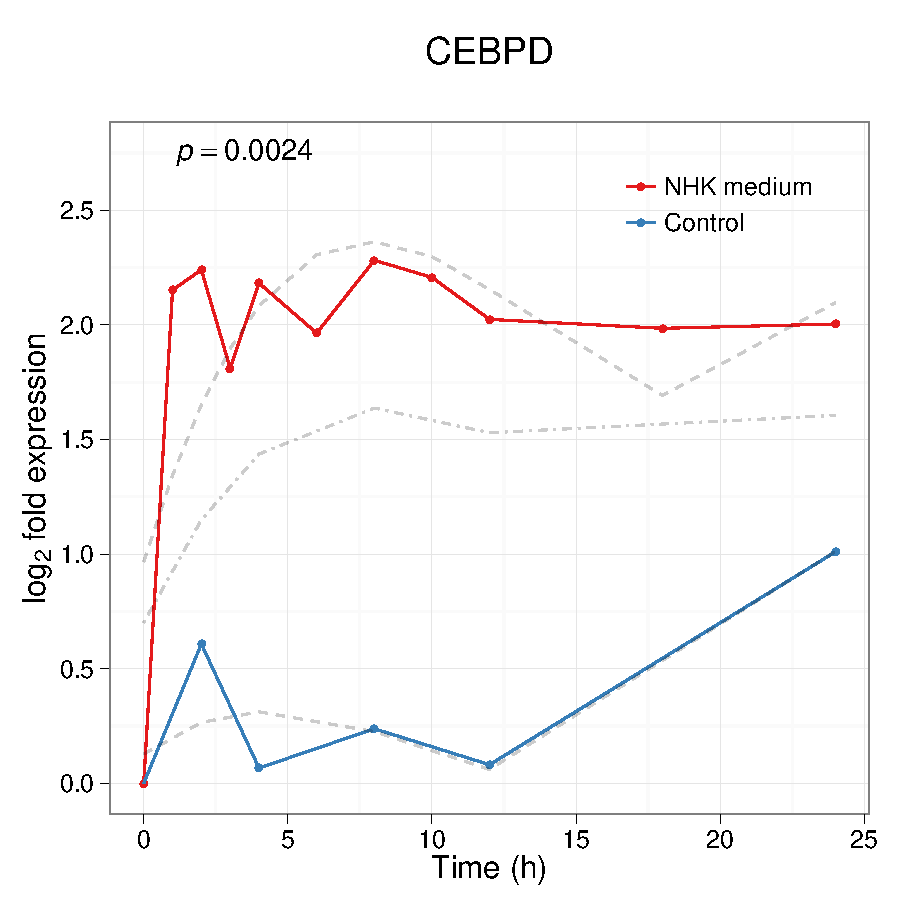
\includegraphics[width=0.8\textwidth]{hdf-fit_cebpd.pdf}
\end{center}
\caption[Full/reduced model fit of gene expression profile]{
{\bf Full/reduced model fit of the expression profile of CEBPD in fibroblasts.}
Shown are the microarray time series under the control and 
keratinocyte-conditioned medium stimulation. Dashed lines indicate the full
model which assumes the alternative hypothesis of differential expression
between conditions; Dot-dashed line represent the reduced model of null 
hypothesis.
}
\label{fig:full_reduced}
\end{figure}

\section{Impulse model}
The qPCR time courses of \tnfa and \sdfonea measured in HPAEC cells are fitted with an impulse model~\cite{Chechik2009}, which is composed of one rising and one falling sigmoidal curve, as defined by
\[
f(x) = \frac{1}{h_1} \cdot \left(h_0+\frac{h_1-h_0}{1+e^{-\beta_1(x-t_1)}}\right) \cdot
\left(h_2+\frac{h_1-h_2}{1+e^{\beta_2(x-t_2)}}\right), 
\]
where the three amplitude (height) parameters determine the initial amplitude 
($h_0$), the peak amplitude
($h_1$), and the steady state amplitude ($h_2$). The onset time $t_1$ is the time of  first transition (inflection point) and the offset $t_2$ is the time of second  transition. Finally, the slope parameters $\beta_1$ and $\beta_2$ determine the slope of the first and second transition. Parameters are estimated using a  Levenberg-Marquardt non-linear least squares  algorithm as implemented in the R package \texttt{minpack.lm}.

\section{Calculating the significantly basal expressed genes}
In order to robustly estimate differentially regulated genes at the basal level and to avoid the commonly encountered 
presence of outliers and skewness~\cite{Marko2011}, we fitted 
a skew-$t$  distribution~\cite{Azzalini2003} to the $\log_2$ raw intensities at 0h. 
In addition to the regular $t$ distribution $f(x)$ with $v_{df}$ degrees of freedom, a skew-$t$ distribution,  $f_{skew}(x)$ has an additional 
skewing parameter $\gamma$ such that  
\[
f_{skew}\left(\frac{x-\xi}{\omega}\right) = 
\begin{cases}
\frac{2\gamma}{\gamma^2+1} \cdot f\left(\gamma\frac{x-\xi}{\omega}\right) & x<0\\
\frac{2\gamma}{\gamma^2+1} \cdot f\left(\frac{1}{\gamma}\frac{x-\xi}{\omega}\right) & x \geqslant 0\\
\end{cases}
\]
where $\xi$  and  $\omega$ denote the location and scale of the distribution.  
The basal level gene expression distribution was fitted using maximum likelihood 
estimation for the 
univariate skew-$t$ distribution, implemented in the R package \texttt{sn}.

%\section{Gene set enrichment analysis}
%\label{sec:h838_gage_table}
%% latex table generated in R 2.15.2 by xtable 1.7-0 package
% Mon Nov 19 15:50:05 2012
\begin{longtable}{rrr}
\caption{Significantly ($p < 0.01$) upregulated gene sets in heterogeneous coculture compared to homogeneous coculture.} \\ 
  \hline
 & p.val & set.size \\ 
  \hline
TIEN\_INTESTINE\_PROBIOTICS\_24HR\_UP & 7.31e-06 & 474 \\ 
   \rowcolor{Gray} SESTO\_RESPONSE\_TO\_UV\_C0 & 2.35e-05 &  98 \\ 
  REACTOME\_CELL\_CYCLE\_MITOTIC & 2.78e-05 & 272 \\ 
   \rowcolor{Gray} REACTOME\_MITOTIC\_M\_M\_G1\_PHASES & 3.61e-05 & 144 \\ 
  HSIAO\_HOUSEKEEPING\_GENES & 4.64e-05 & 356 \\ 
   \rowcolor{Gray} STARK\_PREFRONTAL\_CORTEX\_22Q11\_DELETION\_D & 1.13e-04 & 381 \\ 
  REACTOME\_MITOTIC\_PROMETAPHASE & 1.60e-04 &  82 \\ 
   \rowcolor{Gray} ZHANG\_BREAST\_CANCER\_PROGENITORS\_UP & 2.14e-04 & 331 \\ 
  LI\_WILMS\_TUMOR\_VS\_FETAL\_KIDNEY\_1\_DN & 2.40e-04 & 149 \\ 
   \rowcolor{Gray} OUELLET\_OVARIAN\_CANCER\_INVASIVE\_VS\_LMP\_U & 2.84e-04 & 108 \\ 
  GRAHAM\_CML\_QUIESCENT\_VS\_NORMAL\_QUIESCENT & 3.12e-04 &  76 \\ 
   \rowcolor{Gray} KAUFFMANN\_DNA\_REPAIR\_GENES & 3.32e-04 & 179 \\ 
  PUIFFE\_INVASION\_INHIBITED\_BY\_ASCITES\_UP & 5.04e-04 &  67 \\ 
   \rowcolor{Gray} SHEDDEN\_LUNG\_CANCER\_POOR\_SURVIVAL\_A6 & 5.30e-04 & 389 \\ 
  MISSIAGLIA\_REGULATED\_BY\_METHYLATION\_DN & 5.42e-04 &  87 \\ 
   \rowcolor{Gray} OSMAN\_BLADDER\_CANCER\_UP & 6.26e-04 & 325 \\ 
  KANG\_FLUOROURACIL\_RESISTANCE\_UP & 6.93e-04 &  18 \\ 
   \rowcolor{Gray} REACTOME\_FORMATION\_OF\_ATP\_BY\_CHEMIOSMOTI & 7.68e-04 &  12 \\ 
  REACTOME\_REGULATION\_OF\_GENE\_EXPRESSION\_I & 7.70e-04 &  90 \\ 
   \rowcolor{Gray} REACTOME\_REGULATION\_OF\_BETA\_CELL\_DEVELOP & 8.20e-04 & 100 \\ 
  REACTOME\_FANCONI\_ANEMIA\_PATHWAY & 8.89e-04 &  14 \\ 
   \rowcolor{Gray} REACTOME\_FORMATION\_OF\_A\_POOL\_OF\_FREE\_40S & 9.23e-04 &  85 \\ 
  ROSS\_AML\_OF\_FAB\_M7\_TYPE & 9.46e-04 &  62 \\ 
   \rowcolor{Gray} LENAOUR\_DENDRITIC\_CELL\_MATURATION\_UP & 1.35e-03 &  80 \\ 
  MARTINEZ\_RB1\_AND\_TP53\_TARGETS\_DN & 1.35e-03 & 469 \\ 
   \rowcolor{Gray} LINDGREN\_BLADDER\_CANCER\_CLUSTER\_3\_UP & 1.37e-03 & 273 \\ 
  RUGO\_RESPONSE\_TO\_GAMMA\_RADIATION & 1.38e-03 &  39 \\ 
   \rowcolor{Gray} KYNG\_DNA\_DAMAGE\_BY\_GAMMA\_RADIATION & 1.38e-03 &  39 \\ 
  BARRIER\_CANCER\_RELAPSE\_TUMOR\_SAMPLE\_UP & 1.41e-03 &  14 \\ 
   \rowcolor{Gray} LINDGREN\_BLADDER\_CANCER\_CLUSTER\_1\_DN & 1.50e-03 & 327 \\ 
  SCHWAB\_TARGETS\_OF\_BMYB\_S427G\_DN & 1.51e-03 &  16 \\ 
   \rowcolor{Gray} SCHWAB\_TARGETS\_OF\_BMYB\_I624M\_DN & 1.51e-03 &  16 \\ 
  REACTOME\_CYCLIN\_E\_ASSOCIATED\_EVENTS\_DURI & 1.69e-03 &  54 \\ 
   \rowcolor{Gray} STEIN\_ESRRA\_TARGETS\_RESPONSIVE\_TO\_ESTROG & 1.79e-03 &  36 \\ 
  FLOTHO\_PEDIATRIC\_ALL\_THERAPY\_RESPONSE\_UP & 1.83e-03 &  49 \\ 
   \rowcolor{Gray} FOURNIER\_ACINAR\_DEVELOPMENT\_LATE\_2 & 2.21e-03 & 253 \\ 
  REACTOME\_SCF\_SKP2\_MEDIATED\_DEGRADATION\_O & 2.51e-03 &  48 \\ 
   \rowcolor{Gray} ASTON\_MAJOR\_DEPRESSIVE\_DISORDER\_DN & 2.77e-03 & 140 \\ 
  SENGUPTA\_NASOPHARYNGEAL\_CARCINOMA\_WITH\_L & 2.83e-03 & 300 \\ 
   \rowcolor{Gray} WAKASUGI\_HAVE\_ZNF143\_BINDING\_SITES & 3.21e-03 &  51 \\ 
  ODONNELL\_TARGETS\_OF\_MYC\_AND\_TFRC\_DN & 3.36e-03 &  37 \\ 
   \rowcolor{Gray} VANTVEER\_BREAST\_CANCER\_METASTASIS\_DN & 3.51e-03 &  88 \\ 
  WILCOX\_PRESPONSE\_TO\_ROGESTERONE\_UP & 3.71e-03 & 125 \\ 
   \rowcolor{Gray} CHIANG\_LIVER\_CANCER\_SUBCLASS\_UNANNOTATED & 3.79e-03 &  22 \\ 
  REACTOME\_GENE\_EXPRESSION & 3.85e-03 & 380 \\ 
   \rowcolor{Gray} MUELLER\_COMMON\_TARGETS\_OF\_AML\_FUSIONS\_UP & 3.94e-03 &  12 \\ 
  TAKAO\_RESPONSE\_TO\_UVB\_RADIATION\_UP & 4.24e-03 &  65 \\ 
   \rowcolor{Gray} KEGG\_PROPANOATE\_METABOLISM & 4.38e-03 &  27 \\ 
  BASAKI\_YBX1\_TARGETS\_DN & 4.43e-03 & 271 \\ 
   \rowcolor{Gray} REACTOME\_INSULIN\_SYNTHESIS\_AND\_SECRETION & 4.56e-03 & 117 \\ 
  ROSTY\_CERVICAL\_CANCER\_PROLIFERATION\_CLUS & 4.67e-03 & 128 \\ 
   \rowcolor{Gray} KEGG\_RIBOSOME & 4.95e-03 &  79 \\ 
  REACTOME\_TRANSLATION & 4.96e-03 & 109 \\ 
   \rowcolor{Gray} BERTUCCI\_MEDULLARY\_VS\_DUCTAL\_BREAST\_CANC & 5.16e-03 & 151 \\ 
  KORKOLA\_EMBRYONAL\_CARCINOMA\_UP & 5.17e-03 &  33 \\ 
   \rowcolor{Gray} SMITH\_TERT\_TARGETS\_DN & 5.29e-03 &  66 \\ 
  REACTOME\_SCF\_BETA\_TRCP\_MEDIATED\_DEGRADAT & 5.30e-03 &  44 \\ 
   \rowcolor{Gray} KAYO\_AGING\_MUSCLE\_UP & 5.46e-03 & 152 \\ 
  REACTOME\_SIGNALING\_BY\_WNT & 5.68e-03 &  55 \\ 
   \rowcolor{Gray} MORI\_LARGE\_PRE\_BII\_LYMPHOCYTE\_UP & 5.70e-03 &  51 \\ 
  REACTOME\_PEPTIDE\_CHAIN\_ELONGATION & 5.95e-03 &  76 \\ 
   \rowcolor{Gray} REACTOME\_VIRAL\_MRNA\_TRANSLATION & 5.95e-03 &  76 \\ 
  SPIELMAN\_LYMPHOBLAST\_EUROPEAN\_VS\_ASIAN\_U & 6.09e-03 & 420 \\ 
   \rowcolor{Gray} MARTINEZ\_TP53\_TARGETS\_UP & 6.13e-03 & 485 \\ 
  WALLACE\_PROSTATE\_CANCER\_RACE\_DN & 6.17e-03 &  62 \\ 
   \rowcolor{Gray} NIKOLSKY\_BREAST\_CANCER\_20Q11\_AMPLICON & 6.20e-03 &  27 \\ 
  FLECHNER\_BIOPSY\_KIDNEY\_TRANSPLANT\_REJECT & 6.38e-03 & 484 \\ 
   \rowcolor{Gray} MARTINEZ\_TP53\_TARGETS\_DN & 6.54e-03 & 465 \\ 
  BIOCARTA\_RANMS\_PATHWAY & 6.57e-03 &  10 \\ 
   \rowcolor{Gray} AGUIRRE\_PANCREATIC\_CANCER\_COPY\_NUMBER\_DN & 6.86e-03 & 206 \\ 
  KANG\_IMMORTALIZED\_BY\_TERT\_DN & 6.90e-03 &  91 \\ 
   \rowcolor{Gray} BYSTRYKH\_HEMATOPOIESIS\_STEM\_CELL\_QTL\_CIS & 6.96e-03 &  96 \\ 
  WELCSH\_BRCA1\_TARGETS\_1\_UP & 7.19e-03 & 150 \\ 
   \rowcolor{Gray} MARTORIATI\_MDM4\_TARGETS\_FETAL\_LIVER\_UP & 7.47e-03 &  83 \\ 
  BORCZUK\_MALIGNANT\_MESOTHELIOMA\_UP & 7.47e-03 & 265 \\ 
   \rowcolor{Gray} LE\_EGR2\_TARGETS\_DN & 7.52e-03 &  86 \\ 
  SAKAI\_TUMOR\_INFILTRATING\_MONOCYTES\_UP & 7.80e-03 &  24 \\ 
   \rowcolor{Gray} HADDAD\_T\_LYMPHOCYTE\_AND\_NK\_PROGENITOR\_UP & 7.89e-03 &  67 \\ 
  REACTOME\_FORMATION\_OF\_THE\_TERNARY\_COMPLE & 8.44e-03 &  42 \\ 
   \rowcolor{Gray} BERENJENO\_TRANSFORMED\_BY\_RHOA\_UP & 8.63e-03 & 439 \\ 
  POMEROY\_MEDULLOBLASTOMA\_PROGNOSIS\_DN & 8.72e-03 &  37 \\ 
   \rowcolor{Gray} SENESE\_HDAC1\_TARGETS\_UP & 8.81e-03 & 365 \\ 
  REACTOME\_DIABETES\_PATHWAYS & 9.03e-03 & 333 \\ 
   \rowcolor{Gray} MORI\_EMU\_MYC\_LYMPHOMA\_BY\_ONSET\_TIME\_DN & 9.05e-03 &  16 \\ 
  SANA\_RESPONSE\_TO\_IFNG\_DN & 9.17e-03 &  69 \\ 
   \rowcolor{Gray} DAZARD\_UV\_RESPONSE\_CLUSTER\_G1 & 9.29e-03 &  32 \\ 
  REACTOME\_GTP\_HYDROLYSIS\_AND\_JOINING\_OF\_T & 9.32e-03 &  96 \\ 
   \rowcolor{Gray} LEE\_LIVER\_CANCER\_ACOX1\_UP & 9.46e-03 &  50 \\ 
  CHNG\_MULTIPLE\_MYELOMA\_HYPERPLOID\_DN & 9.50e-03 &  24 \\ 
   \rowcolor{Gray} IIZUKA\_LIVER\_CANCER\_PROGRESSION\_G1\_G2\_DN & 9.57e-03 &  22 \\ 
  BIOCARTA\_BCELLSURVIVAL\_PATHWAY & 9.58e-03 &  11 \\ 
   \rowcolor{Gray}  \hline
\hline
\end{longtable}

%% latex table generated in R 2.15.2 by xtable 1.7-0 package
% Mon Nov 19 15:26:24 2012
\begin{longtable}{rrr}
\caption{Significantly ($p < 0.01$) downregulated gene sets in heterogeneous coculture compared to homogeneous coculture.} \\ 
  \hline
 & p.val & set.size \\ 
  \hline
NAGASHIMA\_NRG1\_SIGNALING\_UP & 2.00e-05 & 144 \\ 
   \rowcolor{Gray} LU\_TUMOR\_VASCULATURE\_UP & 3.23e-05 &  29 \\ 
  NAGASHIMA\_EGF\_SIGNALING\_UP & 2.92e-04 &  49 \\ 
   \rowcolor{Gray} MAHADEVAN\_RESPONSE\_TO\_MP470\_DN & 2.98e-04 &  15 \\ 
  AMIT\_EGF\_RESPONSE\_120\_HELA & 3.91e-04 &  52 \\ 
   \rowcolor{Gray} LU\_TUMOR\_ENDOTHELIAL\_MARKERS\_UP & 5.56e-04 &  22 \\ 
  AMIT\_EGF\_RESPONSE\_20\_HELA & 5.75e-04 &  10 \\ 
   \rowcolor{Gray} NIKOLSKY\_BREAST\_CANCER\_22Q13\_AMPLICON & 5.89e-04 &  13 \\ 
  ENGELMANN\_CANCER\_PROGENITORS\_DN & 2.35e-03 &  55 \\ 
   \rowcolor{Gray} NIKOLSKY\_BREAST\_CANCER\_5P15\_AMPLICON & 2.74e-03 &  18 \\ 
  KEGG\_FRUCTOSE\_AND\_MANNOSE\_METABOLISM & 3.82e-03 &  30 \\ 
   \rowcolor{Gray} NICK\_RESPONSE\_TO\_PROC\_TREATMENT\_DN & 4.00e-03 &  25 \\ 
  LANDIS\_ERBB2\_BREAST\_PRENEOPLASTIC\_UP & 4.34e-03 &  15 \\ 
   \rowcolor{Gray} FRIDMAN\_SENESCENCE\_DN & 4.66e-03 &  12 \\ 
  REACTOME\_PEPTIDE\_LIGAND\_BINDING\_RECEPTORS & 5.78e-03 & 130 \\ 
   \rowcolor{Gray} SHEPARD\_CRUSH\_AND\_BURN\_MUTANT\_UP & 7.17e-03 & 122 \\ 
  GENTILE\_UV\_HIGH\_DOSE\_UP & 7.37e-03 &  12 \\ 
   \rowcolor{Gray} SAGIV\_CD24\_TARGETS\_DN & 7.39e-03 &  40 \\ 
  HOFMANN\_MYELODYSPLASTIC\_SYNDROM\_RISK\_UP & 7.76e-03 &  15 \\ 
   \rowcolor{Gray} BERNARD\_PPAPDC1B\_TARGETS\_UP & 8.96e-03 &  28 \\ 
  AMUNDSON\_GAMMA\_RADIATION\_RESISTANCE & 9.51e-03 &  15 \\ 
   \rowcolor{Gray} BIOCARTA\_RANKL\_PATHWAY & 9.64e-03 &  14 \\ 
   \hline
\hline
\end{longtable}

